\documentclass[10pt]{article}
\usepackage[letterpaper,margin=0.4in]{geometry}
\usepackage[T1]{fontenc}
\usepackage{lmodern}
\usepackage{graphicx}
\usepackage{tabularx}
\usepackage{booktabs}
\usepackage{enumitem}
\usepackage{xcolor}
\usepackage{multicol}
\usepackage{titlesec}

\definecolor{navy}{HTML}{1F3A5F}
\definecolor{soft}{HTML}{EEF2F7}
\titleformat{\section}{\color{navy}\bfseries\normalsize}{}{0pt}{}
\titlespacing*{\section}{0pt}{4pt}{1pt}
\setlist{nosep,leftmargin=1.1em,topsep=1pt}
\setlength{\parindent}{0pt}
\setlength{\parskip}{2pt}
\setlength{\columnsep}{16pt}
\pagestyle{empty}

\begin{document}
\small

{\color{navy}\Large\bfseries Copart, Inc. (NASDAQ: CPRT): Technical Analysis}\hfill{\color{navy}\bfseries\large SHORT}\\[1pt]
{\footnotesize As of Sep 30, 2026 \quad|\quad Price \$27.36 \quad|\quad Entry \$29.19--30.49 \quad|\quad Target \$23.25 \quad|\quad Stop \$32.60 \quad|\quad Reward/risk 2.4x \quad|\quad Horizon 6--12 months}

\vspace{3pt}
\colorbox{soft}{\parbox{\dimexpr\linewidth-2\fboxsep}{\footnotesize
\textbf{Thesis:} The chart shows a de-rating that is not finished. CPRT is 57\% off its May 2025 high, but unlike every earlier drawdown, earnings are shrinking while its main rival, IAA, takes share. A 17.6x P/E looks cheap next to the 34x ten-year median. That is the value trap. We do not short into the \$25.55 floor. We sell rallies into the falling 50-day, stop above it, and target 15x trailing EPS for \textbf{2.4x reward/risk}.}}

\vspace{2pt}
{\centering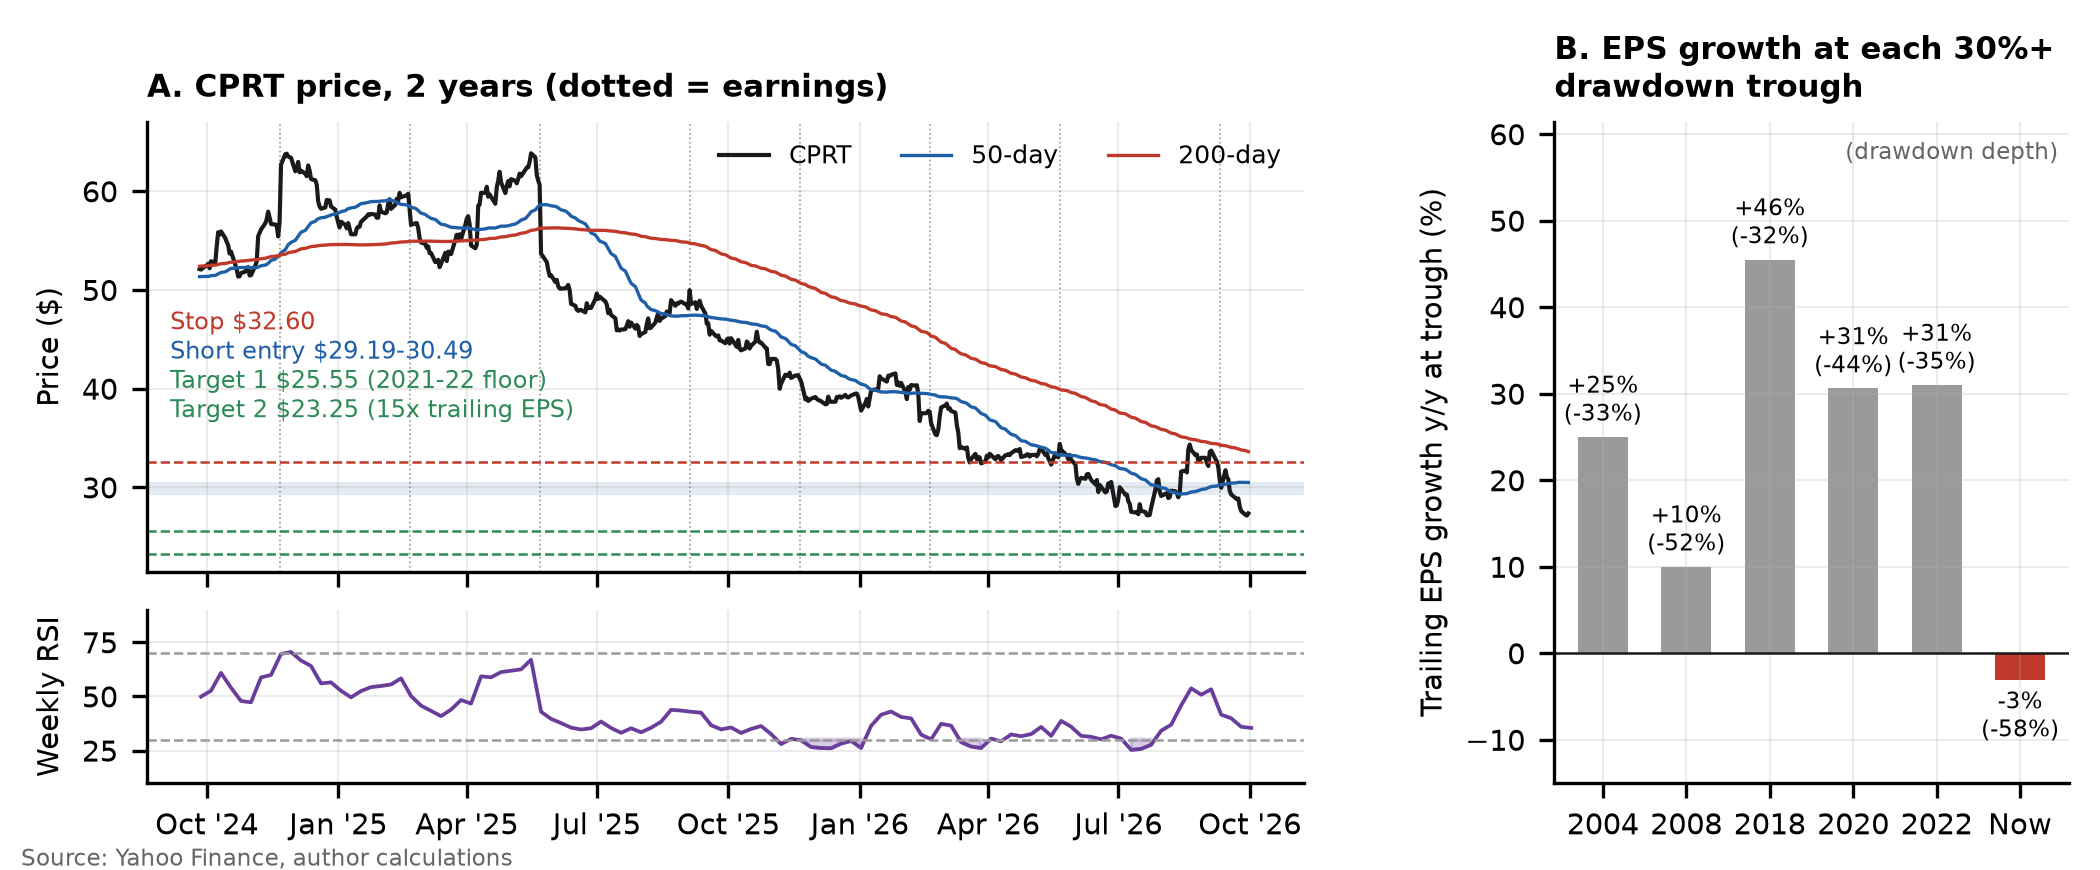
\includegraphics[width=0.76\linewidth]{../model/technicals/output/memo_figure.png}\par}
{\centering\footnotesize\textbf{Exhibit 1.} Price, trend and momentum with the trade levels (A); trailing EPS growth at the trough of every 30\%+ drawdown with EPS data (B).\par}

\begin{multicols}{2}
\section{Setup: a break, not a dip}
\begin{itemize}
  \item \textbf{Deepest drawdown since 2003:} $-$57\% from the May 2025 high. Lowest close since Oct 2022. 340 straight days below a falling 200-day.
  \item \textbf{This time EPS is falling.} In all 5 earlier 30\%+ drawdowns with EPS data, trailing EPS was still up 10--46\%. Today it is $-$3\% (Exhibit 1B).
  \item \textbf{Losing to its rival:} 48 pts behind RB Global (IAA's owner) over 2Y and 56 pts behind the S\&P 500 over 1Y (Exhibit 2C).
\end{itemize}

\section{Evidence: the dips stopped bouncing}
\begin{itemize}
  \item \textbf{Weekly RSI$<$30, 8 signals since 1996:} median 6M return \textbf{$-$0.3\% vs.\ +9.9\%} for all days.
  \item \textbf{Both rallies into the falling 50-day since mid-2025 failed} ($-$16\%, $-$12\% over 3M). Before 2025 the same setup made longs money (+16\% median over 6M, n=23). The regime changed with the fundamentals.
  \item \textbf{Prints disappoint:} the stock fell after 9 of the last 12 reports. The median next-day move on an EPS miss is $-$3.2\% (n=30).
\end{itemize}

\section{Trade plan}
{\footnotesize
\begin{tabularx}{\linewidth}{@{}lrrX@{}}
\toprule
Level & Price & R/R & Basis \\
\midrule
Entry & \$29.19--30.49 & -- & Volume node to falling 50-day \\
Stop & \$32.60 & -- & 1.5 ATR above 50-day / 23.6\% retrace \\
Target 1 & \$26.74 & 1.1x & 52-week low \\
Target 2 & \$25.55 & 1.6x & 2021--22 floor \\
Target 3 & \$23.25 & 2.4x & 15x trailing EPS of \$1.55 \\
\bottomrule
\end{tabularx}}
\begin{itemize}
  \item \textbf{Do not chase:} daily RSI is 32 and price sits on the 2021--22 floor. Wait for the rally.
  \item \textbf{Alternative entry:} if \$25.55 breaks first, short a failed retest of it from below.
\end{itemize}

\section{Fundamental cross-check}
\begin{itemize}
  \item Copart's share of the Copart + IAA salvage pool fell from \textbf{63.9\% to 61.4\%} in FY26. That is about 167k units and \$166M of service revenue.
  \item One lost insurer was $\sim$10\% of U.S. insurance volume. Ex-customer, assignments were +2.3\% vs.\ $-$7.5\% reported.
\end{itemize}

\section{Risks and mitigants}
\begin{itemize}
  \item \textbf{Nov 19 print:} options imply $\pm$10.8\%, wider than the stop. \emph{Mitigant:} half size into the print.
  \item \textbf{Claims recover:} auto insurance CPI is now $-$5.1\% y/y, and cheaper cover could bring back small claims. \emph{Mitigant:} track claim counts monthly and cover if frequency turns up.
  \item \textbf{Buyers step in:} \$1.6B of FY26 buybacks, the ACV deal pitched as growth, and a \$39 Street mean target. \emph{Mitigant:} short interest is only 4.6\% of float (3.3 days to cover), so squeeze risk is low.
\end{itemize}
\textbf{Invalidation:} weekly close above \$32.60, or a reclaim of the 200-day (\$33.61).
\end{multicols}

\vspace{-2pt}
{\centering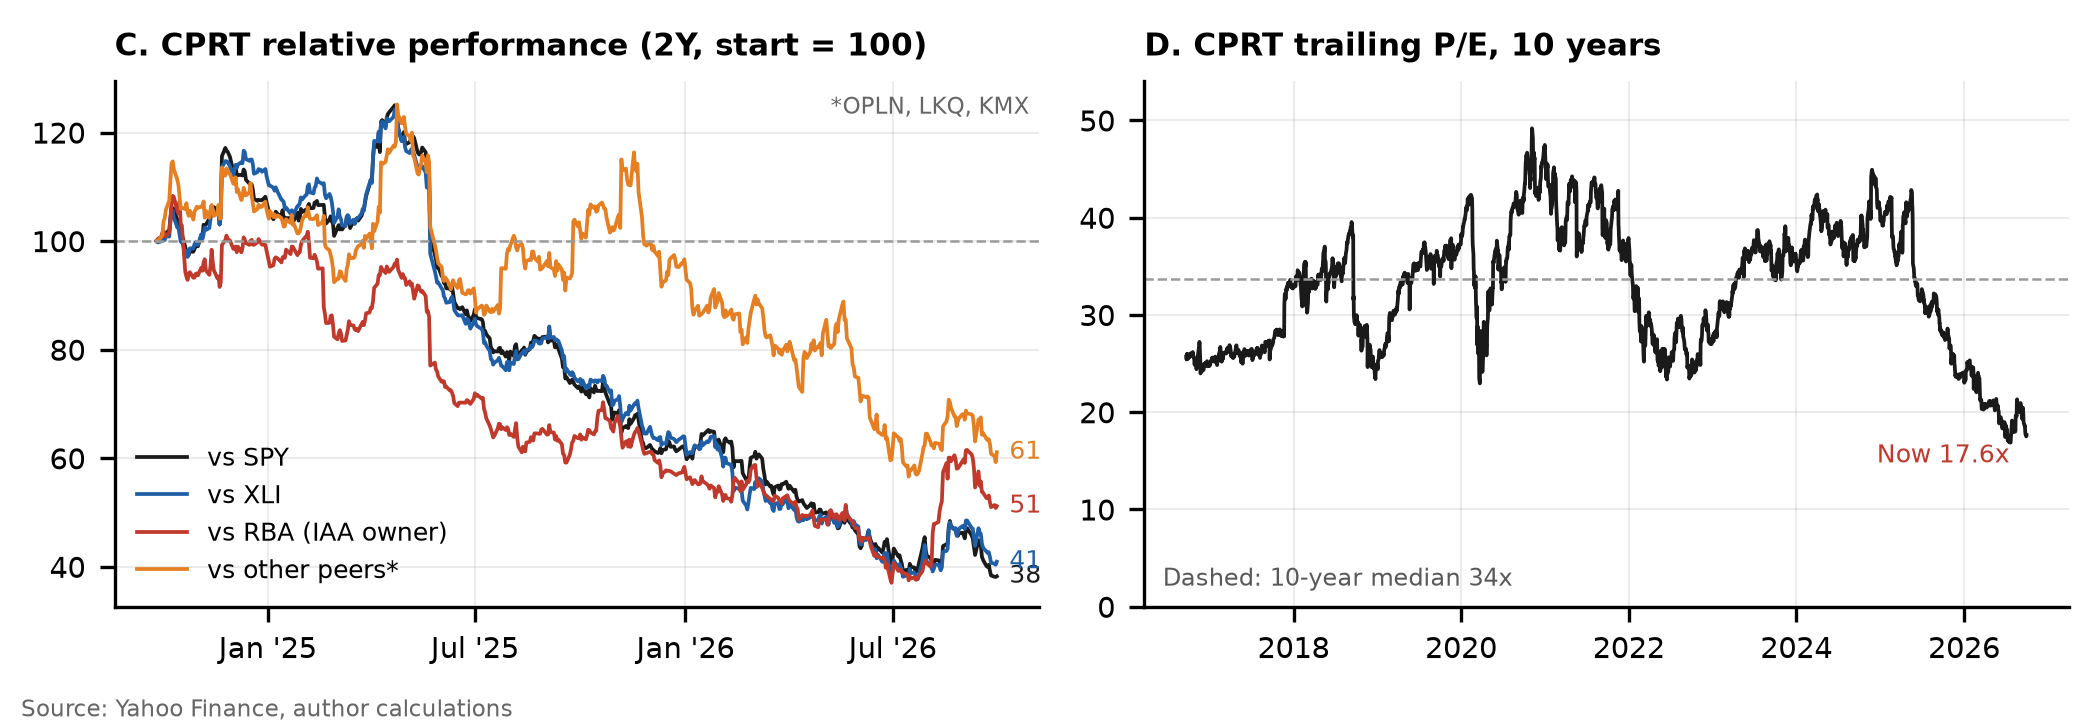
\includegraphics[width=0.68\linewidth]{../model/technicals/output/appendix_figure.png}\par}
{\centering\footnotesize\textbf{Exhibit 2.} CPRT relative to the S\&P 500, industrials, RB Global and other auto remarketing peers (C); trailing P/E over 10 years (D).\par}
{\centering\scriptsize\color{gray} Sources: Yahoo Finance prices, earnings, short interest (Sep 15, 2026) and options; RB Global filings; Copart earnings calls; author calculations. Signal studies use small samples and are context, not proof.\par}
\end{document}
